\section{Durchführung}
  \subsection{Aufbau der Apparatur für niedrige Drücke}
    Im Folgenden wird die Aufbau für einen Druckbereich zwischen $\SI{30}{\milli\bar}$ und etwa $\SI{1000}{\milli\bar}$ näher
    erläutert.
    \begin{figure}
      \centering
      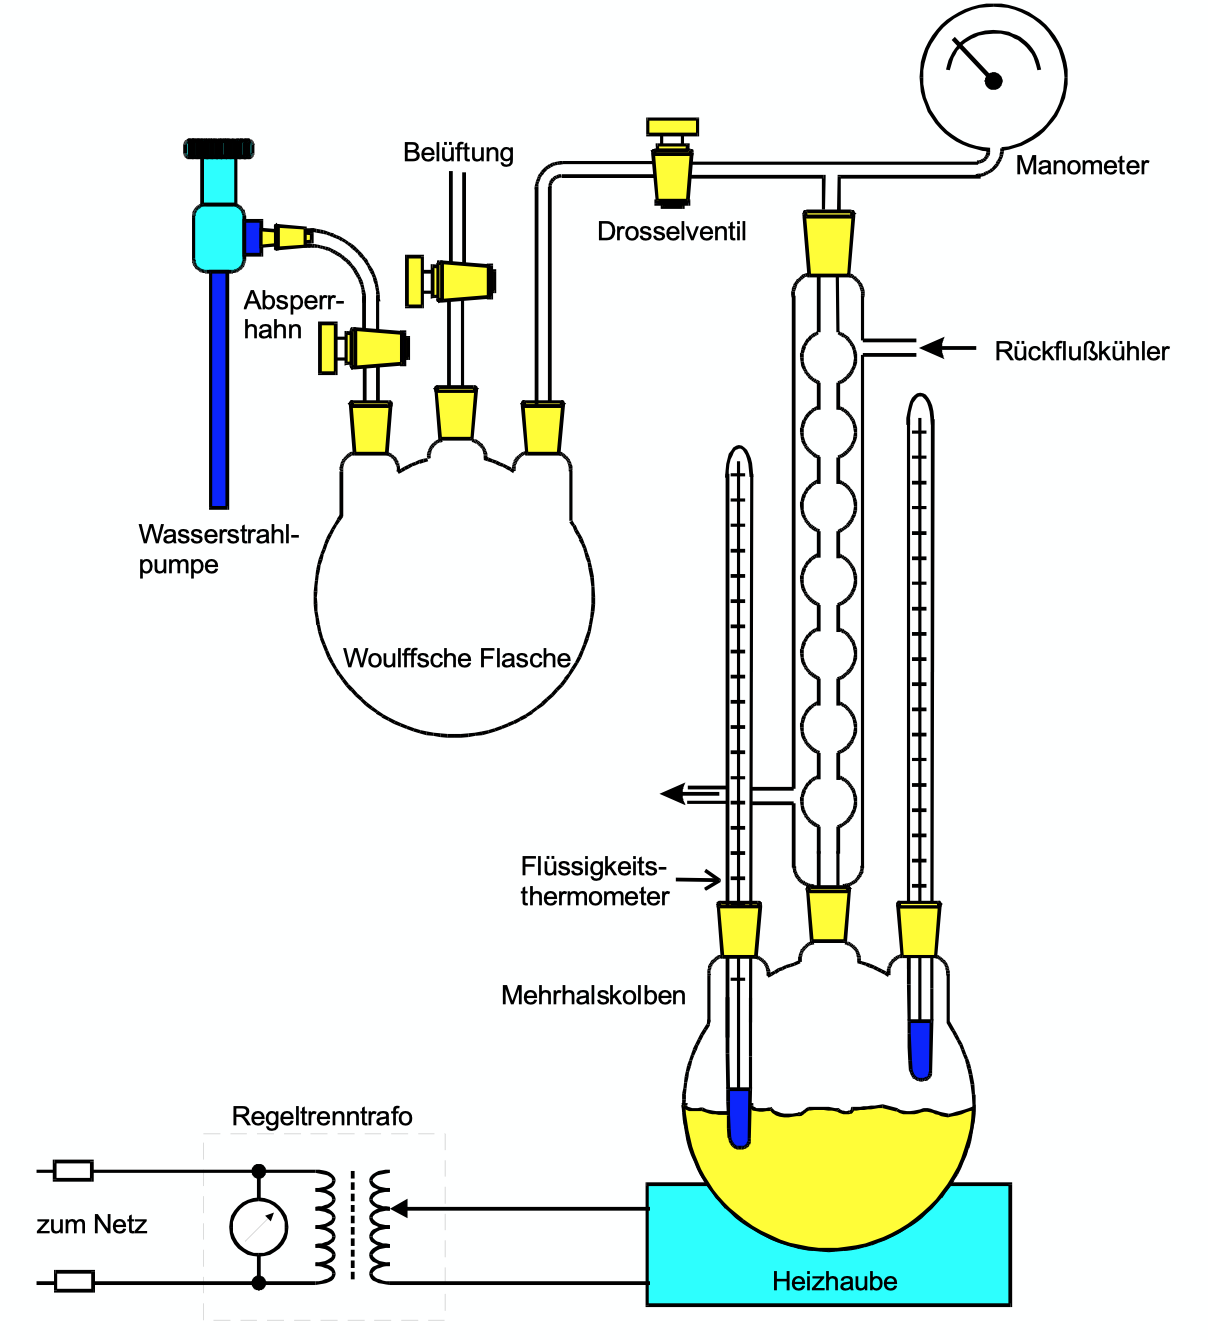
\includegraphics[scale=0.5]{Content/apparaturniedrige.png}
      \caption{Der Versuchsaufbau für den niedrigeren Druckbereich $p \leq \SI{1000}{\milli\bar}$. Quelle: \cite{AP01}}
      \label{fig:niedrigedrücke}
    \end{figure}
    Zu Beginn wird die Apparatur mithilfe einer Wasserstrahlpumpe evakuiert. Absperrhahn und Drosselventil sollten geöffnet und
    das Belüftungsventil geschlossen sein. Nach Erreichen des niedrigsten mit vorhandener Wassertemperatur erreichbaren Druckes
    werden Absperrhahn und Drosselventil wieder geschlossen und die Heizhaube eingeschaltet. Wenn die Flüssigkeit innerhalb
    des Mehrhalskolbens nicht nach kurzer Zeit anfängt zu sieden, kann das Drosselventil zur leichten Senkung des Druckes
    geöffnet werden. Nun lässt sich der Dampfdruck am Manometer sowie die Temperatur am Thermometer ablesen. Wichtig ist, dass
    der Rückflusskühler immer von einer geringen Menge Kühlflüssigkeit durchlaufen wird, sodass die aufsteigenden Dämpfe aus dem
    Mehrhalskolben nicht in das Manometer aufsteigen können, sondern kondensieren und zurück in den Kolben gelangen.
    Die Messungen finden in $\SI{20}{\milli\bar}$-Schritten statt und werden bis zum Erreichen von $\SI{1}{\bar}$ fortgeführt.
    \subsection{Aufbau der Apparatur für höhere Drücke}
    Um Drücke größer als $\SI{1000}{\milli\bar}$ untersuchen zu können, ist \ref{fig:niedrigedrücke} ungeeignet. Daher wird
    hierfür folgender Aufbau verwendet:
    \begin{figure}
      \centering
      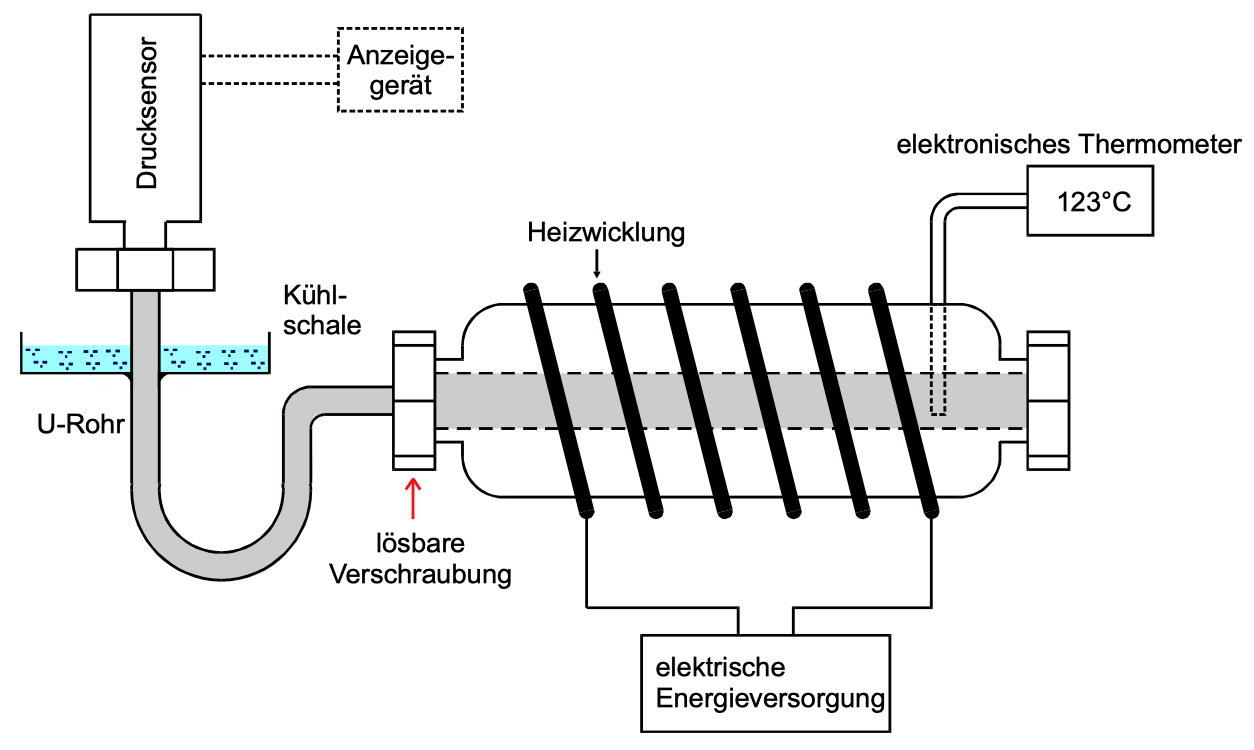
\includegraphics[scale=0.4]{Content/apparaturhohe.png}
      \caption{Der Versuchsaufbau für den höheren Druckbereich $\SI{1}{\bar} \leq p $. Quelle: \cite{AP01}}
      \label{fig:hohedrücke}
    \end{figure}
    Obige Apparatur funktioniert ähnlich zu \ref{fig:niedrigedrücke}, auch hier wird die Flüssigkeit durch eine Wärmequelle
    (hier eine Heizwicklung) erhitzt und es werden mit einem elektrischen Thermometer und einem Drucksensor Datenpaare
    aufgenommen. Hier ist jedoch der Behälter aus Stahl anstelle des Glases gefertigt, um den höheren Drücken wiederstehen zu
    können. Außerdem wird der Drucksensor mittels einer Kühlschale gekühlt. Der Behälter wird mit entgastem und destilliertem
    Wasser gefüllt und fest verschraubt. Die Kühlschale des Drucksensors wird mit einer Kühlflüssigkeit befüllt, woraufhin die
    elektrische Energieversorgung eingeschaltet und die Datenpaare abgelesen werden können. Die Messungen des
    Sättigungsdampfdruckes und der zugehörigen Siedetemperatur finden in $\SI{0.5}{\bar}$-Schritten statt und werden fortgeführt
    bis sich der Drucksensor nahe dem Vollauschlag befindet. Hier wird eine andere Variante der Versuchsapparatur verwendet,
    welche ohne Kühlschale auskommt und ein analoges Thermometer und Manometer besitzt, ansonsten jedoch der obigen Apparatur
    \ref{fig:hohedrücke} gleicht.
\label{sec:Durchführung}
